\documentclass[12pt,oneside,a4paper]{article}

\usepackage[utf8]{inputenc} % Lærer LaTeX at forstå unicode - HUSK at filen skal
% være unicode (UTF-8), standard i Linux, ikke i
% Win.

\usepackage[danish]{babel} % Så der fx står Figur og ikke Figure, Resumé og ikke
% Abstract etc. (god at have).

\usepackage{graphicx}
\usepackage{amsfonts}

%\renewcommand{\mid}[1]{{\rm E}\!\left[#1\right]}
\newcommand{\bas}{\begin{eqnarray*}}
\newcommand{\eas}{\end{eqnarray*}}

\begin{document}

\section{Opgave 1}
Et rektangel $ABCD$ er givet. Vinkelret på diagonalen $AC$ tegnes en linje gennem $D$, som skærer diagonalen i punktet $E$ og som skærer siden $BC$ i punktet $F$.

\begin{figure}[ht]
\begin{center}
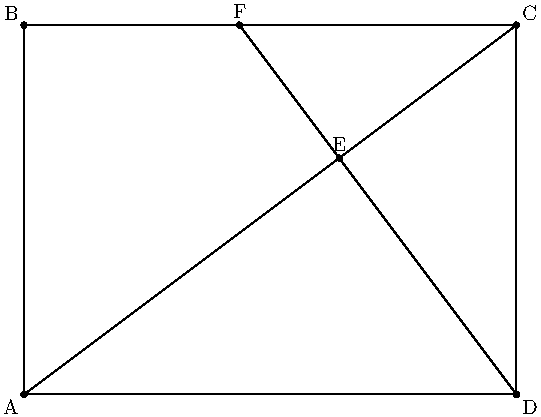
\includegraphics{fig1.pdf}
\label{fig1}
\end{center}
\end{figure}

Det er givet, at arealet af trekant $CEF$ = 2 og arealet af trekant $CED$ = 3. Bestem arealet af firkanten $ABFE$.

\subsection{Løsning}
Trekanterne $FCE$ og $DAE$ er ensvinklede. Der gælder derfor
$$
\frac{|AE|}{|DE|} = \frac{|EC|}{|EF|}
$$
Dette omskrives til
$$
\frac{|AE|}{|EC|} = \frac{|DE|}{|EF|}
$$

Den venstre brøk forlænges med $\frac 12 |DE|$ og den højre brøk forlænges med $\frac 12 |CE|$. Det giver
$$
\frac{\frac 12 |DE| |AE|}{\frac 12 |DE| |EC|} = \frac{\frac 12 |CE| |DE|}{\frac 12 |CE| |EF|}
$$
hvoraf følger følgende sammenhæng mellem arealerne af trekanter.
$$
\frac{\bigtriangleup ADE}{\bigtriangleup CDE} = \frac{\bigtriangleup CDE}{\bigtriangleup CEF}
$$
Med andre ord:
$$
\bigtriangleup ADE = \frac{\left(\bigtriangleup CDE\right)^2}{\bigtriangleup CEF}
$$

Det sidste regnestykke er:
\bas
\Box ABFE &=& \bigtriangleup ABC - \bigtriangleup CEF \\
          &=& \bigtriangleup ACD - \bigtriangleup CEF \\
          &=& \bigtriangleup ADE + \bigtriangleup CDE - \bigtriangleup CEF \\
          &=& \frac{\left(\bigtriangleup CDE\right)^2}{\bigtriangleup CEF} + \bigtriangleup CDE - \bigtriangleup CEF
\eas
Heri indsættes de angive talværdier:
$$
\Box ABFE = \frac{3^2}{2} + 3 - 2 = \frac{11}{2}
$$

\end{document}


